% Theorem T9 Covering using 2-input Multiplexers implementing logic.
%
% OR gate and AND gate implemented using multiplexers form theorem T9.
%
\documentclass[border=3mm]{standalone}
\usepackage{tikz}
\usetikzlibrary{calc,circuits.ee.IEC}

\begin{document}
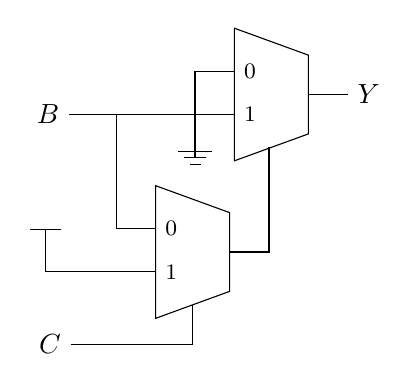
\begin{tikzpicture}[circuit ee IEC,small circuit symbols]

% OR gate implementation with 2-input multiplexer.
% Draw OR mux body.
\draw
    (0,0) coordinate (ORO)
    -- ++ (20:1) coordinate (ORA)
    -- ++ (90:1) coordinate (ORB)
    -- ++ (160:1) coordinate (ORC)
    -- cycle;

% Mux input select.
\draw
    % start in the middle of lower mux body.
    ($(ORO)!0.50!(ORA)$)
    % draw down
    -- ++(270:5mm)
    -- ++(180:15.5mm)
    % label C input select
    node[left]{$C$};

% Loop for each mux terminal.
\foreach \y/\t/\b in {0.1/0/0,0.2/1/1} {

    % Draw each terminal.
    \draw
        ($(ORC)! \y*3.25 !(ORO)$) -- ++(180:0.5cm)
        node(termor\t)[anchor=center] {};

    % Draw binary numbers to select. End loop.
    \draw
        ($(ORC)! \y*3.25 !(ORO)$) ++ (0:0.0)
        node[right,font=\footnotesize] {$\b$};
}

% Draw the VDD symbol to input term0.
\draw
    % start at term0 center
    (termor1.center)
    % these are for some adjustments since we're
    % using this picture as a template.
    -- ++(180:-0.0cm) -- ++(180:9mm)
    % go down
    -- ++(90:5.4mm)
    -- ++(0:2mm) -- ++(180:4mm);

%
% AND gate implementation with 2-input multiplexer.
% Draw AND mux body.
%
\draw
    (1.0,2) coordinate (ANDO)
    -- ++ (20:1) coordinate (ANDA)
    -- ++ (90:1) coordinate (ANDB)
    -- ++ (160:1) coordinate (ANDC)
    -- cycle;

% AND mux output.
\draw
    % Start in middle--this is so clever of tikz!
    ($(ANDA)!0.5!(ANDB)$)
    % draw right
    -- ++(0:5mm)
    % label output on right
    node[right]{$Y$};

% AND mux input select is OR mux output.
\draw
    % start in the middle of lower mux body.
    ($(ANDO)!0.50!(ANDA)$)
    node(andmuxsel){};

% OR mux output.
\draw
    % Start in middle--this is so clever of tikz!
    ($(ORA)!0.5!(ORB)$)
    -- ++(right:5mm) |- (andmuxsel.center);

% Loop for each mux terminal.
\foreach \y/\t/\b in {0.1/0/0,0.2/1/1} {

    % Draw each terminal.
    \draw
        ($(ANDC)! \y*3.25 !(ANDO)$) -- ++(180:0.5cm)
        node(termand\t)[anchor=center] {};

    % Draw binary numbers to select. End loop.
    \draw
        ($(ANDC)! \y*3.25 !(ANDO)$) ++ (0:0.0)
        node[right,font=\footnotesize] {$\b$};
}

% Draw the GND symbol to input term0.
\draw
    % start at term0 center
    (termand0.center)
    % these are for some adjustments since we're
    % using this picture as a template.
    -- ++(180:-0.0cm) -- ++(180:0.0cm)
    % go down
    -- ++(270:1.1)
    % ground symbol
    node[ground={pos=1},point down]{};

% Draw B inputs
\draw
    % start at termor0 center
    (termor0.center)
    % tikz find termand1.center
    |- (termand1.center);
% Complete B input
\draw
    (termand1.center)
    -- ++(180:16mm)
    % label B on left.
    node[left]{$B$};

\end{tikzpicture}
\end{document}
